\documentclass[tikz,border=8pt]{standalone}
% Shared look for every TikZ diagram. Load with \input{../../tools/tikz-style.tex}
\usepackage[T1]{fontenc}
\usepackage{lmodern}
\renewcommand{\sfdefault}{lmr}  % diagrams use the same serif as the text
\usetikzlibrary{arrows.meta, positioning, shapes.geometric, calc, fit, backgrounds}
\definecolor{cblue}{HTML}{4C78A8}
\definecolor{corange}{HTML}{F58518}
\definecolor{cgreen}{HTML}{54A24B}
\definecolor{cred}{HTML}{E45756}
\definecolor{cpurple}{HTML}{B279A2}
\definecolor{cgrey}{HTML}{6B6B6B}
\tikzset{
  every picture/.style={font=\sffamily, line width=1.2pt},
  box/.style={draw=#1, fill=#1!12, rounded corners=4pt, align=center, inner sep=7pt, minimum height=1.1cm},
  box/.default=cgrey,
  arrow/.style={-{Stealth[length=3mm]}, draw=cgrey, line width=1.4pt},
  title/.style={font=\sffamily\bfseries\Large},
  note/.style={font=\sffamily\small, text=cgrey, align=center},
}
\AtBeginDocument{\hyphenpenalty=10000 \exhyphenpenalty=10000}

\begin{document}
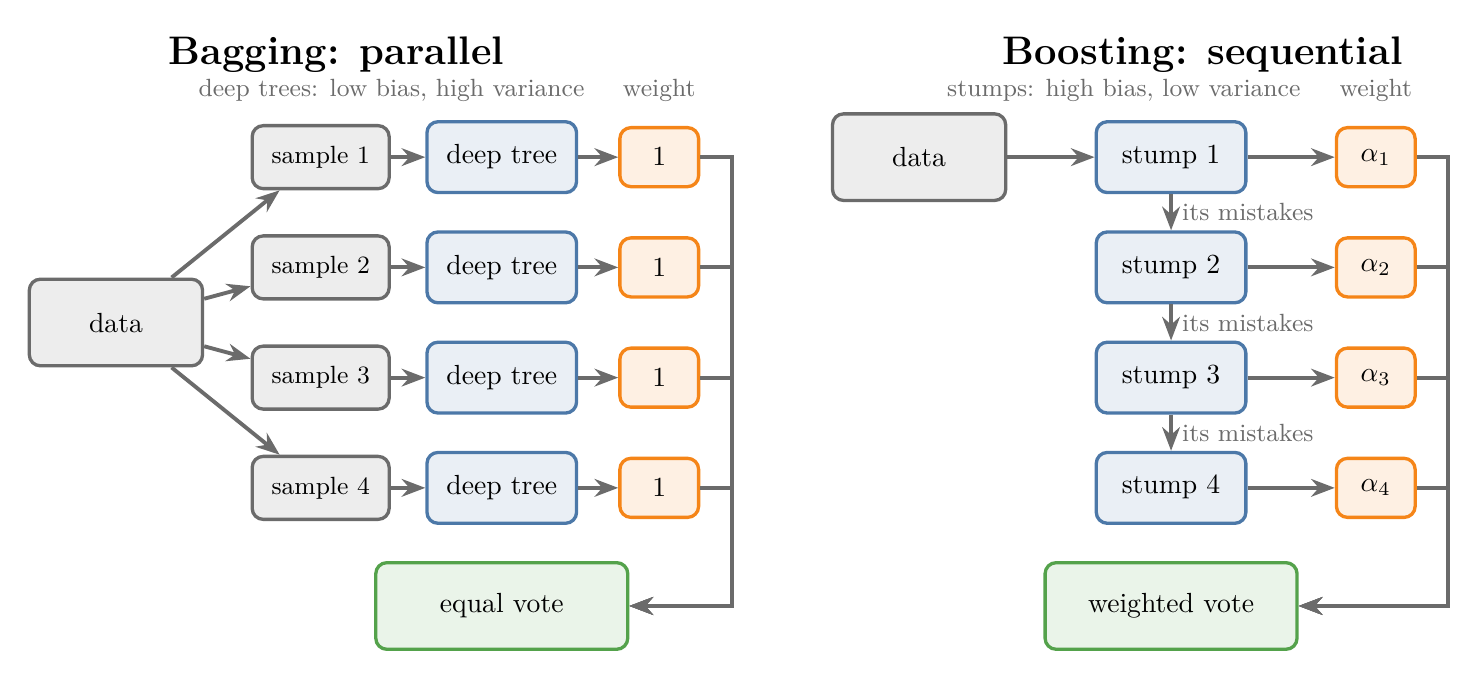
\begin{tikzpicture}[
  d/.style={box=cgrey, minimum width=2.2cm},
  s/.style={box=cgrey, minimum width=1.6cm, minimum height=0.8cm, font=\sffamily\small},
  m/.style={box=cblue, minimum width=1.9cm, minimum height=0.9cm},
  w/.style={box=corange, minimum width=1.0cm, minimum height=0.75cm, inner sep=3pt},
  o/.style={box=cgreen, minimum width=3.2cm}]
  % ---- bagging ----
  \node[title] at (2.8,3.4) {Bagging: parallel};
  \node[d] (D) at (0,0) {data};
  \foreach \i/\y in {1/2.1, 2/0.7, 3/-0.7, 4/-2.1} {
    \node[s] (s\i) at (2.6,\y) {sample \i};
    \node[m] (m\i) at (4.9,\y) {deep tree};
    \node[w] (w\i) at (6.9,\y) {1};
    \draw[arrow] (D) -- (s\i); \draw[arrow] (s\i) -- (m\i); \draw[arrow] (m\i) -- (w\i);
  }
  \node[o] (vb) at (4.9,-3.6) {equal vote};
  \foreach \i in {1,...,4} \draw[arrow] (w\i.east) -- ++(0.4,0) |- (vb.east);
  \node[note] at (6.9,2.95) {weight};
  \node[note] at (3.5,2.95) {deep trees: low bias, high variance};
  % ---- boosting ----
  \begin{scope}[xshift=10.2cm]
  \node[title] at (3.6,3.4) {Boosting: sequential};
  \node[d] (E) at (0,2.1) {data};
  \foreach \i/\y/\a in {1/2.1/0.8, 2/0.7/1.5, 3/-0.7/0.4, 4/-2.1/5.0} {
    \node[m] (b\i) at (3.2,\y) {stump \i};
    \node[w] (a\i) at (5.8,\y) {$\alpha_\i$};
    \draw[arrow] (b\i) -- (a\i);
  }
  \draw[arrow] (E) -- (b1);
  \foreach \i/\j in {1/2, 2/3, 3/4} \draw[arrow] (b\i.south) -- node[note, right] {its mistakes} (b\j.north);
  \node[o] (vs) at (3.2,-3.6) {weighted vote};
  \foreach \i in {1,...,4} \draw[arrow] (a\i.east) -- ++(0.4,0) |- (vs.east);
  \node[note] at (5.8,2.95) {weight};
  \node[note] at (2.6,2.95) {stumps: high bias, low variance};
  \end{scope}
\end{tikzpicture}
\end{document}
